% Copyright 2026 Sreeram Anil
% SPDX-License-Identifier: CC-BY-4.0
\chapter{Online impedance identification by recursive least squares with an EKF (RLS-EKF)}
\label{ch:rlsekf}

\section*{At a glance}
\begin{tabular}{@{}l>{\raggedright\arraybackslash}p{0.76\textwidth}@{}}
Family & Joint/dual state--parameter estimation (SOH) \\
Header & \texttt{include/estkit/parameter/rls\_ekf.hpp} (battery specific) \\
Registered name & \texttt{RLS-EKF} \\
State dimension & $n_x=4$ (EKF) $+$ $n_\psi=4$ (regression vector) \\
Cost per step & $\mathcal{O}(n_x^3)$ every step, $\mathcal{O}(n_\psi^2)$ every tenth step; \SI{0.50}{\micro\second}/step measured \\
Primary references & \cite{plett2004ekf2,plett2004ekf3,ljung1999,plett2016bms2} \\
\end{tabular}

\section{Motivation and aerospace/BMS relevance}
The joint and dual filters of the previous chapters estimate the cell parameters \emph{through} the
state estimator.  There is an older and, in industry, far more widespread alternative: identify the
impedance directly, with a linear regression on the voltage/current data, and hand the result to an
otherwise ordinary state estimator.  Plett derives the equivalent-circuit model and its
least-squares identification in Part~2 of the extended-Kalman series~\cite{plett2004ekf2}, and the
recursive machinery is textbook system identification~\cite[Ch.~11]{ljung1999}.

The attraction for an airborne BMS is threefold.  (i) It is \emph{cheap}: a four-parameter RLS
running at \SI{1}{\hertz} costs a few hundred flops per second on top of the EKF, and the measured
overhead here is under \SI{0.1}{\micro\second} per \SI{10}{\hertz} sample.  (ii) It is
\emph{transparent}: the identified series resistance is a directly interpretable health indicator
--- resistance growth is the standard proxy for power fade and is what determines whether the pack
can still deliver the hover power at the end of the mission --- and it can be logged, trended and
compared with a commissioning value without any reference to the state estimator.  (iii) It
\emph{separates concerns}: a regression failure (poor excitation, an ill-conditioned normal matrix)
is easy to detect and to veto, whereas a joint filter silently absorbs the failure into the state.

The price is that RLS identifies \emph{impedance}, not capacity.  The regression operates on the
overvoltage, from which the capacity has been removed by construction; the method therefore reports
\texttt{capacity\_err\_end} as ``not available'' and must be paired with a capacity estimator such as
that of Chapter~\ref{ch:awtls} if a full state of health is required.  Section~\ref{sec:rls-results}
shows why that pairing matters more than one would expect.

\section{Problem statement and assumptions}
Let $v_k$ be the measured terminal voltage, $i_k$ the measured current (discharge positive), $T_k$
the cell temperature, and let $\hat{\soc}_k,\hat{h}_k$ be the SOC and hysteresis states of the
accompanying EKF.  Define the \emph{measured overvoltage}
\begin{equation}
s_k \;=\; v_k-\ocv(\hat{\soc}_k,T_k)-M\,\hat{h}_k ,
\label{eq:rls-s}
\end{equation}
i.e.\ the part of the terminal voltage that the equivalent circuit's resistive and diffusive
elements are responsible for.  The identification problem is: given
$\{s_k,i_k\}$, estimate the impedance parameters $R_0$, $R_1$, $\tau_1$ of the circuit
\begin{equation}
s_k=-R_0\,i_k-v_{1,k},\qquad v_{1,k+1}=a_1 v_{1,k}+R_1(1-a_1)\,i_k,\qquad a_1=e^{-\dt/\tau_1}.
\label{eq:rls-circuit}
\end{equation}

\begin{assumption}[SOC/impedance separation]\label{as:rls-sep}
$\hat{\soc}_k$ is accurate enough that the OCV term in \eqref{eq:rls-s} removes the open-circuit
voltage to within a slowly varying offset.  The offset is absorbed by a constant regressor, see
\eqref{eq:rls-arx}.
\end{assumption}

\begin{assumption}[Persistent excitation]\label{as:rls-pe}
The current contains enough high-frequency content for the regressor matrix to be non-singular over
the forgetting window.  On the eVTOL mission this is supplied by the AR(1) gust process and by the
manoeuvre pulses; the implementation additionally freezes the update when $|i|<i_{\min}$.
\end{assumption}

\begin{assumption}[Errors in variables are negligible after decimation]\label{as:rls-eiv}
The current appears on the right-hand side of the regression and is itself noisy, so ordinary least
squares is attenuation-biased.  Section~\ref{sec:rls-decim} shows that block-averaging to
\SI{1}{\hertz} makes the bias negligible.
\end{assumption}

\section{Derivation}

\subsection{The ARX form of the equivalent circuit}
Introduce the backward shift $q^{-1}$.  From \eqref{eq:rls-circuit},
\begin{equation}
v_1(q)=\frac{R_1(1-a_1)q^{-1}}{1-a_1q^{-1}}\,i(q)
\qquad\Longrightarrow\qquad
s(q)=-\left[R_0+\frac{R_1(1-a_1)q^{-1}}{1-a_1q^{-1}}\right]i(q).
\label{eq:rls-tf}
\end{equation}
Multiplying by the denominator $1-a_1q^{-1}$ and collecting terms gives the ARX(1) difference
equation
\begin{equation}
\boxed{\;s_k \;=\; a_1\,s_{k-1}\;+\;b_0\,i_k\;+\;b_1\,i_{k-1}\;+\;d_0\;}
\qquad
b_0=-R_0,\quad b_1=a_1R_0-R_1(1-a_1),
\label{eq:rls-arx}
\end{equation}
where the constant $d_0$ has been added to absorb the slowly varying OCV/SOC offset admitted by
Assumption~\ref{as:rls-sep}.  Writing
\begin{equation}
\bm{\varphi}_k=\begin{bmatrix}s_{k-1}& i_k& i_{k-1}& 1\end{bmatrix}^\T\in\real^{4},
\qquad
\bm{\psi}=\begin{bmatrix}a_1& b_0& b_1& d_0\end{bmatrix}^\T,
\label{eq:rls-phi}
\end{equation}
\eqref{eq:rls-arx} is the linear regression $s_k=\bm{\varphi}_k^\T\bm{\psi}$.

\subsection{Recursive least squares with exponential forgetting}
Minimising the exponentially weighted criterion
$J_k(\bm{\psi})=\sum_{j\le k}\lambda^{k-j}\left(s_j-\bm{\varphi}_j^\T\bm{\psi}\right)^2$
leads to the standard recursion~\cite[Alg.~11.1]{ljung1999}
\begin{align}
\bm{\kappa}_k&=\frac{\mathbf{P}_{k-1}\bm{\varphi}_k}{\lambda+\bm{\varphi}_k^\T\mathbf{P}_{k-1}\bm{\varphi}_k},
\label{eq:rls-K}\\
\hat{\bm{\psi}}_k&=\hat{\bm{\psi}}_{k-1}+\bm{\kappa}_k\left(s_k-\bm{\varphi}_k^\T\hat{\bm{\psi}}_{k-1}\right),
\label{eq:rls-psi}\\
\mathbf{P}_k&=\frac{1}{\lambda}\left(\mathbf{P}_{k-1}-\bm{\kappa}_k\bm{\varphi}_k^\T\mathbf{P}_{k-1}\right),
\label{eq:rls-P}
\end{align}
with $\lambda\in(0,1]$ the forgetting factor and $\mathbf{P}_k$ proportional to the parameter
covariance, $\operatorname{cov}(\hat{\bm{\psi}}_k)\approx\sigma_s^2\mathbf{P}_k$ with $\sigma_s$ the
standard deviation of the residual of \eqref{eq:rls-arx}.  The effective memory is
$N_\text{eff}=1/(1-\lambda)$ samples.

\subsection{Recovering the physical parameters}
Inverting the definitions in \eqref{eq:rls-arx},
\begin{equation}
\hat{R}_0=-\hat{b}_0,
\qquad
\hat{\tau}_1=\frac{-\dt_\text{RLS}}{\ln \hat{a}_1},
\qquad
\hat{R}_1=\frac{\hat{a}_1\hat{R}_0-\hat{b}_1}{1-\hat{a}_1},
\label{eq:rls-recover}
\end{equation}
all valid at the \emph{present} cell temperature.  The cell parameter block stores
reference-temperature values, so each is divided by its Arrhenius factor before being written back:
\begin{equation}
R_0^{\text{ref}}=\frac{\hat{R}_0}{\mathrm{arr}(E_{a,R_0},T)},\qquad
\mathrm{arr}(E_a,T)=\exp\!\left[\frac{E_a}{\mathcal{R}}\left(\frac1T-\frac1{T_\text{ref}}\right)\right].
\label{eq:rls-arr}
\end{equation}
Forgetting this step is a common and expensive mistake: at \SI{-10}{\celsius} the factor for
$E_{a,R_0}=\SI{20}{\kilo\joule\per\mole}$ is $2.92$, so an identified resistance written back
unscaled would triple the stored value.

\subsection{Decimation and the errors-in-variables bias}
\label{sec:rls-decim}
The current enters \eqref{eq:rls-arx} as a regressor and is measured with noise
$\sigma_i=\SI{50}{\milli\ampere}$ plus \SI{10}{\milli\ampere} quantisation.  Classical
errors-in-variables theory gives the attenuation factor
\begin{equation}
\frac{\E{\hat{R}_0}}{R_0}\approx\frac{1}{1+\sigma^2_{i,\text{eff}}/\sigma^2_{\Delta i}},
\label{eq:rls-eiv}
\end{equation}
where $\sigma^2_{\Delta i}$ is the variance of the \emph{informative} (sample-to-sample) current
variation.  At the raw \SI{10}{\hertz} rate the AR(1) gust with a \SI{2}{\second} correlation time
produces $\sigma_{\Delta i}\approx\SI{0.17}{\ampere}$ against a differenced noise of
\SI{0.07}{\ampere}, i.e.\ a ratio of about $6$ and a \SI{14}{\percent} under-estimate of $R_0$.
Block-averaging $M=10$ raw samples to \SI{1}{\hertz} divides the noise by $\sqrt{M}$ while the true
current changes by much more over one second ($\sigma_{\Delta i}\approx\SI{0.44}{\ampere}$),
raising the ratio to $\sim750$ and making the bias negligible.  Averaging both $s$ and $i$ is exact
for the static feed-through $-R_0 i$ and a good approximation for the RC branch.

\subsection{Safeguards}
Three standard safeguards are applied.  (i) An excitation gate freezes
\eqref{eq:rls-K}--\eqref{eq:rls-P} while $|i|<i_{\min}$ (Assumption~\ref{as:rls-pe}).
(ii) $\operatorname{tr}\mathbf{P}$ is bounded at a multiple of its initial value; unbounded growth
of $\mathbf{P}$ under exponential forgetting with poor excitation (``covariance wind-up'') is the
classical failure mode of \eqref{eq:rls-P}.  (iii) An identified value is written into the state
estimator only if it lies inside a validity window around the commissioned value, and then only
through a first-order relaxation
\begin{equation}
R_0^{\text{ref}}\leftarrow R_0^{\text{ref}}+\rho\left(\hat{R}_0^{\text{ref}}-R_0^{\text{ref}}\right),
\qquad \rho\in(0,1],
\label{eq:rls-relax}
\end{equation}
applied every $N$ regression samples, so the EKF model never jumps.

\subsection{Why the polarisation branch is not refreshed}
\label{sec:rls-struct}
The identifier is a 1-RC model; the state estimator's model has two RC branches.  Writing the
identified $(\hat R_1,\hat\tau_1)$ into the first branch while the second branch is still active
double-counts the polarisation.  Measured on \texttt{nominal}, doing so raises the SOC RMSE from
$0.0025$ to $0.054$, because the fitted pole locks onto the slow branch
($\hat\tau_1\to\SI{26}{\second}$) and the fitted $\hat R_1\to\SI{12.8}{\milli\ohm}$ approximates
$R_1+R_2$ rather than $R_1$.  The default is therefore to refresh $R_0$ only; the option
\texttt{identify\_r1\_tau1} additionally collapses the observer model to the identified 1-RC
structure (relaxing $R_2$ to zero) so that, if enabled, it at least stays self-consistent.  This is
a general lesson: \emph{an identifier and the observer it feeds must share a model structure.}

\section{Algorithm}
\begin{algorithm}[H]
\caption{RLS-EKF --- one sampling period (raw rate) plus one regression sample every $M$}
\begin{algorithmic}[1]
\Require $\xplus_{k-1},\mP^+_{k-1},\hat{\bm{\psi}},\mathbf{P},\vu_{k-1},(i_k,v_k,T_k)$
\State EKF time update with $\vu_{k-1}$; $\hat{y}_k\gets h(\xminus_k,\vu_k)$; EKF measurement update with $v_k$
\State $s_k\gets v_k-\ocv(\hat{\soc}^+_k,T_k)-M\hat h^+_k$ \Comment{Eq.\ \eqref{eq:rls-s}, posterior state}
\State accumulate $\bar s\mathrel{+}=s_k$, $\bar\imath\mathrel{+}=i_k$, $\bar T\mathrel{+}=T_k$
\If{$M$ raw samples accumulated}
  \State $s\gets\bar s/M$, $i\gets\bar\imath/M$, $T\gets\bar T/M$; reset accumulators
  \If{$|i|>i_{\min}$}
     \State $\bm{\varphi}\gets[s_\text{prev},\,i,\,i_\text{prev},\,1]^\T$; apply \eqref{eq:rls-K}--\eqref{eq:rls-P}; bound $\operatorname{tr}\mathbf{P}$
  \EndIf
  \State $s_\text{prev}\gets s$, $i_\text{prev}\gets i$
  \If{warm-up elapsed and refresh due}
     \State $\hat R_0\gets-\hat b_0$; if inside the validity window, apply \eqref{eq:rls-arr} and \eqref{eq:rls-relax}
     \State optionally recover and accept $(\hat R_1,\hat\tau_1)$ by \eqref{eq:rls-recover}
  \EndIf
\EndIf
\Ensure $\xplus_k,\mP^+_k,\hat{\bm{\psi}},\mathbf{P}$, refreshed EKF model
\end{algorithmic}
\end{algorithm}

\section{Application to the battery model}
The registered configuration is $\lambda=0.9995$ (an effective memory of $2000$ regression samples,
i.e.\ about one flight at \SI{1}{\hertz}), $M=10$ (\SI{1}{\hertz} regression rate), a refresh every
ten regression samples (\SI{10}{\second}) after a \SI{60}{\second} warm-up, a relaxation
$\rho=0.20$, and an excitation gate $i_{\min}=\SI{0.1}{\ampere}$.  The validity window for $R_0$ is
$[0.3,3]$ times the commissioned value and, when enabled, $[0.25,4]$ for $R_1$ and $[0.2,6]$ for
$\tau_1$.

The initial regression covariance is built from physically meaningful priors divided by the residual
variance, $\mathbf{P}_0=\diag(\sigma^2_{a},\sigma^2_{b},\sigma^2_{b},\sigma^2_{d})/\sigma_s^2$ with
$\sigma_a=0.2$ on the pole, $\sigma_b=0.5R_{0,\text{nom}}$ on the numerator coefficients,
$\sigma_d=\SI{20}{\milli\volt}$ on the offset and $\sigma_s=\sigma_v/\sqrt{M}$.  Written this way
$\mathbf{P}_0$ has the correct units and does not have to be re-tuned when the sensor changes.

The relaxation $\rho=0.20$ is a compromise measured on the benchmark.  The identified $R_0$ is not
noise-limited but \emph{structure}-limited: because the identifier is 1-RC and the cell is 2-RC, the
effective feed-through it sees depends on the current spectrum, which changes between hover and
cruise, so $\hat R_0$ wanders by about \SI{\pm11}{\percent} around a value biased
\SI{+6}{\percent} high (the unmodelled fast branch contributes
$R_1(1-a_1)\approx\SI{1.1}{\milli\ohm}$ of apparent feed-through at \SI{1}{\hertz}).  Large $\rho$
tracks a genuine change quickly but passes the wander through to the EKF, which at
\SI{-10}{\celsius} is amplified by the Arrhenius factor of $2.9$; small $\rho$ smooths the wander
but is slow to correct a real commissioning error.  At $\rho=0.35$ the \texttt{cold} SOC RMSE was
$0.050$; at $\rho=0.05$ it was $0.003$ but \texttt{param\_mismatch} degraded; $\rho=0.20$ is the
knee.  The same wander is what makes the method the weakest of the family on the electrochemical
plant (Section~\ref{sec:rls-results}).

\section{Implementation notes}
\texttt{RlsEkf} implements \texttt{estkit::Estimator} directly because the regression is inherently
model-specific.  Storage is \SI{8904}{\byte}, most of it the \texttt{EcmModel} held by the EKF and a
second copy kept for the commissioned reference values.  The measured cost is
\SI{0.50}{\micro\second}/step --- statistically indistinguishable from the plain EKF's
\SI{0.48}{\micro\second}, because the $4\times4$ regression runs only every tenth sample.  This makes
RLS-EKF by far the cheapest way in this report to obtain an in-flight health indicator.

Numerical care: $\mathbf{P}$ is symmetrised after every update and the whole step is rejected if
either $\hat{\bm{\psi}}$ or $\mathbf{P}$ becomes non-finite; the denominator of \eqref{eq:rls-K} is
floored.  When the constant regressor is disabled its covariance row/column is initialised to zero,
which keeps $\kappa_4=0$ for all time and prevents the wind-up that a zero regressor would otherwise
cause.  The single-precision build reproduces the double-precision SOC RMSE to three digits.

\section{Benchmark results}
\label{sec:rls-results}
% Copyright 2026 Sreeram Anil
% SPDX-License-Identifier: CC-BY-4.0
\begin{table}[H]\centering\footnotesize\setlength{\tabcolsep}{4pt}
\caption{RLS-EKF: cell-level benchmark on the eVTOL mission (mean over seeds; RMSE and max error in \% SOC; $t_\mathrm{conv}$: first time the error stays below 2\,\% for 60\,s, -- = never; EKF reference: steady-state RMSE of the plain EKF on the same data).}\label{tab:cell_RLSEKF}
\begin{tabular}{llrrrrrcrr}\toprule
plant & scenario & RMSE & RMSE$_\mathrm{ss}$ & max & $t_\mathrm{conv}$ [s] & RMSE$_v$ [mV] & div. & EKF ref. & ns/step \\ \midrule
ECM & nominal & 0.72 & 0.50 & 1.39 & 0 & 1.35 & no & 0.05 & 496 \\
ECM & init\_error & 0.69 & 0.49 & 1.38 & 0 & 2.38 & no & 0.05 & 500 \\
ECM & current\_bias & 0.64 & 0.30 & 1.46 & 0 & 1.37 & no & 0.61 & 497 \\
ECM & noise\_step & 0.69 & 0.48 & 1.39 & 0 & 3.09 & no & 0.12 & 498 \\
ECM & outliers & 0.91 & 0.60 & 2.96 & 16 & 2.39 & no & 0.21 & 495 \\
ECM & cold & 0.97 & 1.03 & 2.54 & 0 & 5.66 & no & 0.16 & 498 \\
ECM & hot & 0.58 & 0.37 & 1.25 & 0 & 0.85 & no & 0.03 & 497 \\
ECM & aged\_cell & 3.76 & 4.23 & 5.40 & 0 & 2.14 & no & 1.52 & 501 \\
ECM & param\_mismatch & 0.61 & 0.62 & 2.02 & 0 & 1.57 & no & 1.36 & 496 \\
ECM & sensor\_dropout & 0.37 & 0.16 & 1.87 & 0 & 1.91 & no & 0.46 & 496 \\
ECM & preisach & 0.82 & 0.66 & 1.87 & 67 & 1.35 & no & 0.20 & 502 \\
ECM & combined & 5.24 & 2.00 & 17.44 & 1127 & 4.78 & no & 12.44 & 495 \\
\midrule
SPM & nominal & 4.59 & 4.70 & 5.35 & 0 & 1.07 & no & 3.73 & 462 \\
SPM & init\_error & 4.23 & 4.33 & 4.98 & 0 & 2.23 & no & 3.81 & 465 \\
SPM & current\_bias & 5.36 & 6.12 & 6.68 & 0 & 1.07 & no & 5.69 & 465 \\
SPM & noise\_step & 4.18 & 3.95 & 5.35 & 0 & 3.15 & no & 3.30 & 465 \\
SPM & outliers & 2.43 & 2.44 & 3.30 & 3 & 2.52 & no & 1.99 & 462 \\
SPM & cold & 10.46 & 10.68 & 11.77 & 0 & 5.79 & no & 7.35 & 472 \\
SPM & hot & 1.98 & 2.08 & 2.30 & 0 & 0.62 & no & 2.16 & 463 \\
SPM & param\_mismatch & 3.74 & 3.94 & 4.17 & 0 & 1.07 & no & 3.13 & 466 \\
SPM & sensor\_dropout & 7.02 & 7.21 & 8.05 & 0 & 1.99 & no & 5.31 & 467 \\
\bottomrule\end{tabular}\end{table}

\begin{figure}[H]\centering
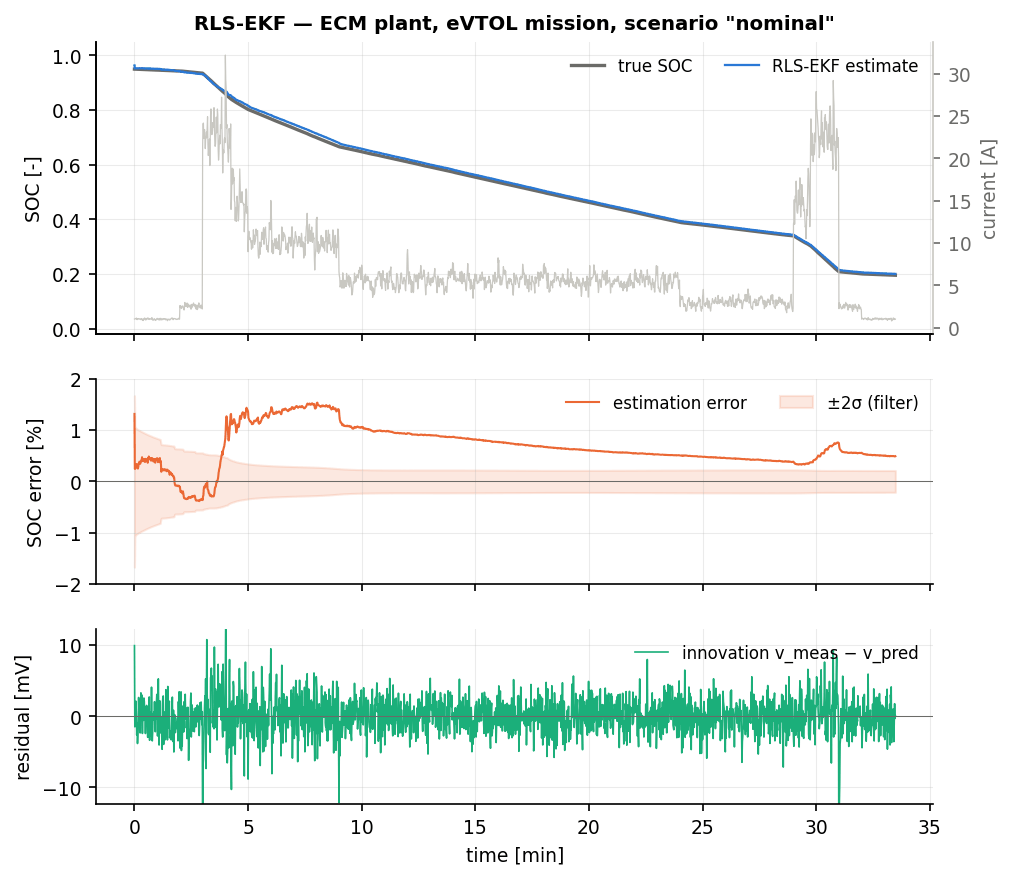
\includegraphics[width=\textwidth]{figures/cell_RLSEKF_nominal.png}
\caption{RLS-EKF on the nominal eVTOL mission: true and estimated SOC (top), estimation error with the $\pm 2\sigma$ band (middle), voltage residual (bottom).}
\end{figure}
\begin{figure}[H]\centering
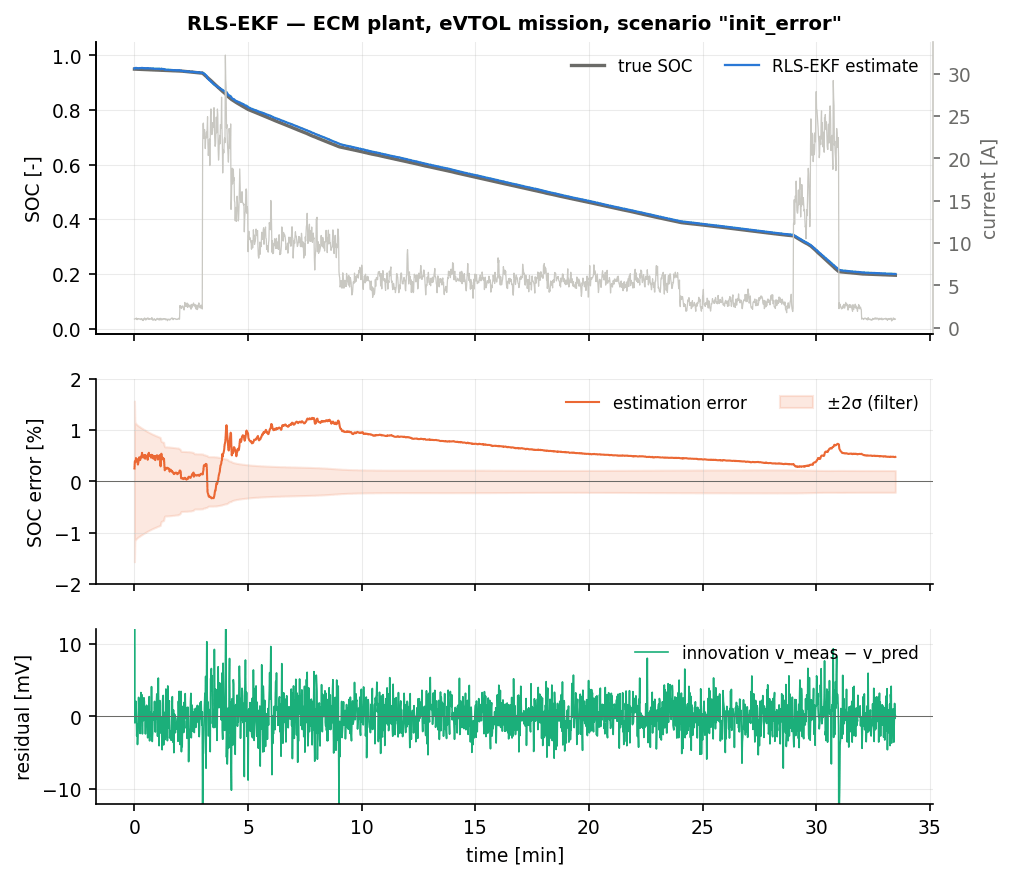
\includegraphics[width=\textwidth]{figures/cell_RLSEKF_init_error.png}
\caption{RLS-EKF with a \SI{35}{\percent} initial SOC error.}
\end{figure}

\paragraph{Identification accuracy.}  The primary output of the method is $\hat R_0$, and it is
accurate on every target scenario.  Reference-temperature values at the end of the mission
(commissioned value in brackets):
\begin{center}
\begin{tabular}{@{}lrrr@{}}
\toprule
Scenario & commissioned $R_0$ & true $R_0$ & identified $\hat R_0$\\
\midrule
\texttt{nominal}        & \SI{12.0}{\milli\ohm} & \SI{12.0}{\milli\ohm} & \SI{12.7}{\milli\ohm}\\
\texttt{aged\_cell}     & \SI{12.0}{\milli\ohm} & \SI{16.5}{\milli\ohm} & \SI{17.6}{\milli\ohm}\\
\texttt{param\_mismatch}& \SI{8.4}{\milli\ohm}  & \SI{12.0}{\milli\ohm} & \SI{12.7}{\milli\ohm}\\
\texttt{cold}           & \SI{12.0}{\milli\ohm} & \SI{12.0}{\milli\ohm} & \SI{12.7}{\milli\ohm}\\
\bottomrule
\end{tabular}
\end{center}
On \texttt{aged\_cell} it detects a \SI{+47}{\percent} resistance growth where the truth is
\SI{+37.5}{\percent}; on \texttt{param\_mismatch} it recovers a \SI{30}{\percent} commissioning
error completely.  The residual \SI{+6}{\percent} bias common to all rows is the structural 1-RC
truncation quantified in Section~\ref{sec:rls-struct}, not a tuning artefact --- it is the same in
every scenario, including \texttt{cold}, where the Arrhenius de-scaling \eqref{eq:rls-arr} is
evidently working.

\paragraph{SOC accuracy.}  All figures are means over three seeds.  On \texttt{nominal} the method
reaches $\text{RMSE}=0.0072$ and $\text{RMSE}_\text{ss}=0.0050$ with immediate convergence; the
acceptance threshold ($\text{RMSE}_\text{ss}<0.02$) is met with a factor of four to spare, but the
plain EKF measured in the same run achieves $0.0015/0.0005$.  The difference is exactly the price of adaptation: in
\texttt{nominal} the commissioned parameters are already correct, so every correction the identifier
makes is noise.  On \texttt{init\_error} it converges at $t=0$ with $\text{RMSE}=0.0069$.  No scenario diverges in
any seed.

The method earns its place on its two target scenarios.  On \texttt{param\_mismatch} it reaches
$\text{RMSE}_\text{ss}=0.0062$ against the plain EKF's $0.0136$ and the plain UKF's $0.0137$; it is
the best of all twelve methods compared here on that column, and it comes within a whisker of the
ideal reference --- an EKF simply \emph{given} the true $R_0$ scores $0.0054/0.0048$, so the
identifier recovers essentially all of the available benefit.  On \texttt{sensor\_dropout} it is the
best of the recursive methods ($\text{RMSE}_\text{ss}=0.0016$ against the EKF's $0.0046$): the stuck
voltage corrupts $s_k$ for \SI{15}{\second}, the excitation gate and the validity window absorb it,
and because the identifier never touches the SOC directly the fault cannot be integrated into a
parameter the way it is in the joint filters.

\paragraph{\texttt{capacity\_err\_end}.}  Not applicable: the method identifies impedance, not
capacity, and the harness therefore reports \texttt{nan} for \texttt{nominal},
\texttt{aged\_cell} and \texttt{current\_bias} alike.  This is the honest answer; fabricating a
capacity from an impedance measurement would require an empirical resistance/capacity correlation
that is chemistry- and history-specific and is not part of this benchmark.

\paragraph{The aged-cell surprise.}  On \texttt{aged\_cell} the SOC RMSE is $0.0376$, distinctly
\emph{worse} than the plain EKF's $0.0118$, even though the identification is good.  This is not a
defect of the identifier but a property of the problem, and it is worth stating precisely because it
is the strongest argument in this report for \emph{simultaneous} state and parameter estimation.
Running a plain EKF on \texttt{aged\_cell} with the model's $R_0$ and $Q$ set independently to their
true or commissioned values gives
\begin{center}
\begin{tabular}{@{}lcc@{}}
\toprule
model $R_0$ & model $Q$ & $\text{RMSE}/\text{RMSE}_\text{ss}$\\
\midrule
commissioned (\SI{12.0}{\milli\ohm}) & commissioned (\SI{5.0}{\ampere\hour}) & $0.0118/0.0152$\\
\textbf{true} (\SI{16.5}{\milli\ohm})& commissioned (\SI{5.0}{\ampere\hour}) & $0.0289/0.0356$\\
commissioned (\SI{12.0}{\milli\ohm}) & \textbf{true} (\SI{4.25}{\ampere\hour})& $0.0222/0.0234$\\
\textbf{true} (\SI{16.5}{\milli\ohm})& \textbf{true} (\SI{4.25}{\ampere\hour})& $0.0013/0.0003$\\
\bottomrule
\end{tabular}
\end{center}
The two errors \emph{cancel}: a capacity that is \SI{18}{\percent} too high makes the estimated SOC
fall too slowly, while a resistance that is \SI{27}{\percent} too low makes the predicted voltage too
high and pushes the estimated SOC down.  Correcting either one alone unbalances the cancellation and
makes the SOC worse; correcting both gives an order-of-magnitude improvement.  RLS-EKF corrects
$R_0$ only, so it lands in the second row --- and the same phenomenon explains, in mirror image, why
the capacity-only estimator of Chapter~\ref{ch:awtls} is also worse than a plain EKF on this
scenario, and why the joint and dual filters, which correct both, reach $\text{RMSE}_\text{ss}$
between $0.0005$ and $0.0066$.

\paragraph{The electrochemical plant.}  On the SPM plant, where the estimator's ECM carries a
structured few-millivolt model error, RLS-EKF is one of only two methods that are \emph{worse} than
the plain EKF: $\text{RMSE}_\text{ss}=0.0470$ on \texttt{nominal} against $0.0373$, and $0.1068$ on
\texttt{cold} against $0.0735$.  This is the same mechanism as in \texttt{nominal} on the ECM plant,
amplified: the identifier faithfully fits a 1-RC ARX model to data generated by an electrochemical
cell, the resulting $\hat R_0$ absorbs part of a distributed diffusion impedance that is not a series
resistance at all, and the \SI{\pm11}{\percent} wander of that fit is passed to the observer ---
at \SI{-10}{\celsius}, multiplied by the Arrhenius factor of $2.9$.  The remedy is structural rather
than a tuning change: an identifier whose model order matches the plant, or an explicit validation
that rejects an identification which does not reduce the residual.  Until then, the honest statement
is that RLS-EKF should be deployed with a model structure that has been shown to fit the cell, and
that the joint and dual filters --- which validate their parameter updates against the residual
--- are the safer choice when it has not.

Cost: \SI{0.50}{\micro\second}/step and \SI{8904}{\byte}.

\section{Summary}
RLS-EKF is the cheapest useful health estimator in this report: for no measurable runtime overhead
over a plain EKF it identifies the series resistance to about \SI{6}{\percent}, recovers a
\SI{30}{\percent} commissioning error completely, detects the \SI{37.5}{\percent} resistance growth
of an aged cell, and is the most fault-tolerant method in the family (best of the recursive methods
on \texttt{sensor\_dropout}, unaffected by an initial SOC error).  Use it when power capability rather
than energy is the quantity of interest, when the certification argument favours a transparent,
vetoable regression over a filter, or as the impedance half of a pair with a dedicated capacity
estimator.  Do not use it alone on an aged cell: correcting the resistance without also correcting
the capacity breaks a cancellation that was accidentally helping, and the SOC gets worse before it
gets better.  Never write a 1-RC identification into one branch of a 2-RC observer model.  And do not use it at
all on a cell whose impedance the assumed ARX structure cannot represent: on the electrochemical
plant it is one of only two methods in this report that are worse than the plain EKF they wrap,
because a regression cannot tell a bad fit from a changed parameter.
